%%% ==========================================================================
%%% Evidence-Grounded Automated Forecasting for Enterprise Sales Data
%%% IEEEtran conference paper.
%%%
%%% Build:
%%%     pdflatex main
%%%     bibtex   main
%%%     pdflatex main
%%%     pdflatex main
%%%
%%% Requires: IEEEtran.cls, and the standard packages loaded below.
%%% Figures are in ./figures as PDF; the bibliography is ./references.bib.
%%% ==========================================================================
\documentclass[conference]{IEEEtran}

% IEEEtran_HOWTO: with the conference option IEEEtran already sets the two
% column layout, margins, fonts and section numbering required by IEEE.
% No margin, font size, column width or spacing parameter is overridden
% anywhere in this file.

\usepackage{cite}
\usepackage{amsmath,amssymb}
\usepackage{graphicx}
\usepackage{booktabs}
\usepackage{array}
\usepackage{url}
\usepackage{textcomp}

% IEEEtran_HOWTO recommends loading hyperref last, if it is used at all.
\usepackage[hidelinks]{hyperref}

\graphicspath{{figures/}}

% Correct bad hyphenation here.
\hyphenation{fore-cast-ing walk-for-ward con-for-mal}

\begin{document}

\title{Evidence-Grounded Automated Forecasting for\\Enterprise Sales Data: Grain Selection,\\Leakage-Free Validation and Conformal Reliability}

% ---------------------------------------------------------------------------
% AUTHOR BLOCK
% TODO before submission: replace the department, institution and location
% below with the real values. (Note: a line that begins with "[" immediately
% after "\\" would be parsed as \\'s optional length argument, so do not
% wrap placeholders in square brackets here.)
% ---------------------------------------------------------------------------
\author{\IEEEauthorblockN{Vedant Kokate}
\IEEEauthorblockA{\textit{Department of Data Science}\\
\textit{Institution Name}\\
City, Country\\
vedshlokgk@gmail.com}}

\maketitle

% ===========================================================================
\begin{abstract}
Enterprise resource planning (ERP) systems hold the transactional history a
business needs to forecast its own revenue, but that history arrives with
cryptic column names, recycled identifiers, irregular invoice arrivals and no
declared forecasting frequency. Automated forecasting tools assume this work
has already been done, so in practice the accuracy figures they report are
shaped less by the model than by decisions taken before any model is fitted.
This paper presents and empirically evaluates an end-to-end forecasting
pipeline that treats those decisions as first-class, measurable components:
semantic resolution of ERP column names, composite-key transaction identity,
selection of the forecast \emph{grain} from structural evidence rather than
from transaction inter-arrival time, a single shared walk-forward fold plan
evaluated at the deployment horizon with all preprocessing fitted inside each
fold, and split-conformal prediction intervals whose coverage is measured
prequentially and reported alongside a six-factor reliability rating that is
explicitly not a probability. The pipeline is evaluated on a four-year ERP
export of 392 invoices, 21 columns and 59.2 million INR of net sales. Grain
selection rejects the weekly grain that inter-arrival inference implies
(84.7\% observed-period density, best model 69.03\% WAPE) in favour of a
monthly grain (100\% density, 47.48\% WAPE). Under an identical 11-fold plan,
simple exponential smoothing (47.48\% WAPE) outperforms SARIMA (67.66\%) and
XGBoost (62.44\%), and none of 15 feature-engineered machine-learning
configurations beats it by the 1~pp threshold set for a separable
improvement. Two evaluation choices are shown to matter more than model
choice: a single trailing hold-out reports 11.52\% WAPE for the model that
ranks seventh of eight under walk-forward validation (rank correlation
$\rho=-0.381$, $p=0.352$), and fitting preprocessing on the whole series
before splitting understates error by 2.91--6.28~pp across models. The
published 80\% intervals attain 66.7\% prequential coverage on 21
out-of-sample points, which the system reports as a calibration deficit
rather than concealing.
\end{abstract}

\begin{IEEEkeywords}
sales forecasting, enterprise resource planning, automated machine learning,
time series cross-validation, data leakage, conformal prediction, forecast
evaluation, schema matching
\end{IEEEkeywords}

% ===========================================================================
\section{Introduction}

Revenue forecasting is one of the few analytical tasks almost every
organisation performs, and the data required for it already exists inside the
enterprise resource planning (ERP) system that records each invoice. The
distance between having that data and having a trustworthy forecast is
nevertheless substantial, and most of it lies outside the forecasting model.
An ERP export arrives as a flat table with abbreviated column names
(\texttt{nsv}, \texttt{inv\_dt}, \texttt{disc\_pct}), identifiers that are
reused rather than unique, missing values scattered across business fields,
and no statement anywhere of the temporal frequency at which the underlying
demand should be modelled. Every one of these must be resolved before a model
can be fitted, and each resolution is a modelling decision in its own right.

The forecasting literature has established, repeatedly and across very large
benchmarks, that the marginal return from model sophistication on short
business series is small. The M4 and M5 competitions and the controlled
comparisons that accompanied them show that simple statistical methods and
their combinations remain difficult to beat, that machine-learning methods
require substantially more data and computation to compete, and that
uncertainty quantification is at least as hard as point
accuracy~\cite{makridakis2018statml,makridakis2022m5acc,makridakis2022m5unc,spiliotis2022sku}.
The same literature has been equally clear that measurement choices --- the
evaluation protocol, the error measure, the treatment of the train/test
boundary --- can dominate the differences being
measured~\cite{tashman2000outofsample,bergmeir2012cv,hyndman2006accuracy,kolassa2020bestpoint}.

Automated forecasting systems, however, largely begin downstream of these
concerns. Automated pipelines and AutoML forecasting libraries take a clean,
correctly indexed series as input and automate what happens
afterwards~\cite{meisenbacher2022pipelines,shchur2023autogluon}; feature-based
meta-learners select or weight models from series features computed on a
series that is assumed to already
exist~\cite{monteromanso2020fforma,talagala2023fforms}. The steps that turn an
ERP table into that series --- which column is revenue, which rows are the
same transaction, at what period demand should be aggregated --- are treated
as preprocessing and left to the practitioner, even though on a short business
series they can change the answer more than the choice of model does.

This paper reports the design and empirical evaluation of a pipeline built on
the opposite premise: that on enterprise sales data of realistic size, the
decisions preceding the model, and the protocol used to measure the model,
should be made explicit, automated, and evaluated with the same rigour as the
forecast itself. Concretely:

\begin{itemize}
\item \textbf{Forecast grain is selected, not inherited.} Transaction
      inter-arrival time measures how often a business raises invoices, not
      the period at which its demand is forecastable. Four candidate grains
      are scored on structural evidence (observed-period density, history
      length, dispersion, seasonal support, resolution) computed on a leading
      training span only, with no model fitted and no forecast error consulted.
\item \textbf{One validation protocol, shared by every candidate.} A single
      expanding-origin walk-forward plan is derived once from the series and
      applied to every model, at the production horizon, with outlier capping
      and gap bridging refitted inside each fold and forecasts scored against
      raw actuals.
\item \textbf{Uncertainty is estimated from out-of-sample error and audited.}
      Prediction intervals are split-conformal quantiles of the relative
      errors the winning model actually produced across folds; their coverage
      is measured prequentially and their sharpness by the Winkler score.
\item \textbf{Reported confidence is evidence, not probability.} A six-factor
      reliability rating aggregates accuracy, fold-to-fold consistency,
      history, input quality, interval calibration and selection margin, and
      states explicitly that it is not a probability of correctness.
\end{itemize}

The contribution is empirical and architectural rather than algorithmic. No
new forecasting algorithm is proposed. What is new is the demonstration, on a
real ERP export, that (i) the grain decision alone moves best-achievable
error from 69.03\% to 47.48\% WAPE, (ii) the evaluation protocol changes which
model is declared best in a way that is not merely a matter of degree, and
(iii) a system that measures and reports its own calibration deficit is
attainable at negligible additional cost. Section~\ref{sec:related} surveys the
relevant literature; Section~\ref{sec:gap} states the gap;
Section~\ref{sec:method} describes the pipeline; Sections~\ref{sec:setup}
and~\ref{sec:results} give the experimental setup and results;
Sections~\ref{sec:discussion}--\ref{sec:conclusion} discuss, bound and
conclude.

% ===========================================================================
\section{Related Work}
\label{sec:related}

\subsection{What large-scale evidence says about model choice}

The M-competition series provides the most reliable available evidence about
which forecasting methods work on business data at scale. The M5 accuracy
competition, run on 42{,}840 Walmart retail series, found that top submissions
improved substantially over the organisers' statistical benchmarks, but that
those improvements diminished at lower levels of the hierarchy where series
are short and noisy~\cite{makridakis2022m5acc}. On the 1{,}045 monthly M3
series, machine-learning methods were dominated by statistical methods across
accuracy measures and horizons, at considerably greater computational
cost~\cite{makridakis2018statml}. A controlled comparison on daily SKU demand
reached a compatible conclusion: machine learning helps when there is enough
data and cross-series structure to exploit, and hurts when there is
not~\cite{spiliotis2022sku}. The comprehensive review by Petropoulos
\emph{et al.}~\cite{petropoulos2022theory} places these findings in a broader
methodological context.

For the individual-company series considered here --- a single series of tens
of periods, no cross-series pool --- this literature predicts that
low-parameter exponential smoothing should be competitive and that heavily
parameterised models should not. Our results in
Section~\ref{sec:results} are consistent with that prediction, which is why we
treat the finding as confirmation rather than novelty.

\subsection{Automatic model selection and AutoML for forecasting}

Automatic forecasting has a long statistical lineage: the ETS state-space
framework made exponential smoothing model selection an information-criterion
problem~\cite{hyndman2002statespace}, and the \texttt{forecast} package made
automatic ETS/ARIMA selection routine~\cite{hyndman2008forecastpkg}.
Feature-based meta-learning generalised the idea by mapping series features to
a model choice (FFORMS~\cite{talagala2023fforms}) or to combination weights
(FFORMA~\cite{monteromanso2020fforma}), both trained across large reference
collections. Modern AutoML forecasting libraries such as
AutoGluon--TimeSeries~\cite{shchur2023autogluon} automate model search,
ensembling and probabilistic output; the review of automated forecasting
pipelines by Meisenbacher \emph{et al.}~\cite{meisenbacher2022pipelines}
catalogues the design space.

Two properties of this body of work matter here. First, every method takes a
constructed series as its input; the feature vector FFORMS classifies, or the
frame AutoGluon ingests, presupposes that frequency, aggregation and record
identity are settled. Second, meta-learners derive their mapping from a large
external corpus of series, which is exactly what a single organisation
forecasting its own revenue does not have. Our selection stage therefore uses
the series' own out-of-sample evidence rather than a learned prior, which is
weaker in principle but available in practice.

\subsection{Evaluation protocol, leakage and error measures}

Tashman's review of out-of-sample testing established rolling-origin
evaluation as the standard for honest forecast
assessment~\cite{tashman2000outofsample}, and Bergmeir and Ben\'itez showed
empirically that blocked/ordered cross-validation is preferable to a single
hold-out for time-series predictor evaluation, whose estimates are noisy and
sensitive to where the split
falls~\cite{bergmeir2012cv}. Kaufman \emph{et al.}~\cite{kaufman2012leakage}
formalised leakage as the introduction of information about the target that
would not be legitimately available at prediction time, and identified
preprocessing fitted before splitting as a canonical instance.

On error measures, Hyndman and Koehler~\cite{hyndman2006accuracy} catalogued
the failure modes of percentage errors when actuals approach zero and proposed
scaled alternatives; Davydenko and Fildes~\cite{davydenko2013measuring} showed
that averaging per-point ratios is unsuitable for SKU-level demand and
advocated aggregate (ratio-of-sums) measures; Kolassa~\cite{kolassa2020bestpoint}
demonstrated that different measures are minimised by different point
forecasts, so the measure is part of the specification, not a neutral readout.
These three results motivate our use of the weighted absolute percentage
error (WAPE) as the primary ranking metric and the deliberate exclusion of
MAPE from any ranking decision.

\subsection{Uncertainty quantification}

Conformal prediction provides distribution-free finite-sample coverage under
exchangeability~\cite{vovk2005conformal}, with split-conformal regression
bands developed by Lei \emph{et al.}~\cite{lei2018distfree}. Time series
violate exchangeability, which has motivated dedicated constructions; EnbPI
attains approximately valid marginal coverage for strongly mixing errors
without data splitting or exchangeability~\cite{xu2021enbpi}. Evaluation of
interval forecasts rests on proper scoring
rules~\cite{gneiting2007scoring}, of which the Winkler interval
score~\cite{winkler1972interval} is the standard instance for a central
interval, penalising width so that coverage cannot be bought by widening
alone. The M5 uncertainty competition demonstrated how much harder
distributional accuracy is than point accuracy in
retail~\cite{makridakis2022m5unc}. Our intervals are split-conformal quantiles
of relative errors drawn from walk-forward folds --- a pragmatic instance of
this family whose exchangeability assumption we test empirically rather than
assume, and report against.

\subsection{Temporal aggregation}

The level of temporal aggregation is known to change which components of a
series are visible and how accurately it can be forecast. Temporal
hierarchies~\cite{athanasopoulos2017temporal} reconcile forecasts produced at
several aggregation levels, improving accuracy and robustness. That literature
establishes the premise on which our grain stage rests --- that aggregation
level is a modelling decision with measurable consequences --- while
addressing a different problem: it reconciles across levels given a
hierarchy, whereas the question in an ERP export is which single level should
be modelled at all when none is declared.

\subsection{Preparing the table: schema, identity, quality}

Automatic schema matching has been surveyed since Rahm and
Bernstein~\cite{rahm2001schema}, whose taxonomy separates schema-level from
instance-level and element-level from structure-level matchers. Learned
semantic type detection (Sherlock~\cite{hulsebos2019sherlock}) predicts a
column's semantic type from its values, and general-purpose text embedding
models such as E5~\cite{wang2022e5} provide strong sentence-level
representations usable for matching column names against a business glossary.
Record-level identity is a separate and well-studied problem: the duplicate
record detection survey of Elmagarmid
\emph{et al.}~\cite{elmagarmid2007duplicate} covers similarity metrics and
algorithms for approximate duplicates. Our pipeline combines a rule
dictionary with E5 embeddings for column mapping and a composite business key
for record identity; neither is novel as a technique, but both are load-bearing
for the forecast, and Section~\ref{sec:results} quantifies what happens when
identity is resolved incorrectly.

\subsection{Positioning}

Table~\ref{tab:related} summarises where existing work operates relative to
the decisions this paper studies. The pattern is consistent: the forecasting
literature analyses these decisions in isolation and rigorously, while the
automation literature builds systems that assume them already made.

\begin{table}[!t]
\caption{Which of the four pre-model decisions the core method of each cited
line of work explicitly addresses. \textmd{$\bullet$~addressed as part of the
method; $\circ$~assumed given or out of scope. The assessment concerns the
cited papers' own contributions, not what their surrounding software
ecosystems can be made to do.}}
\label{tab:related}
\centering
\footnotesize
\setlength{\tabcolsep}{4pt}
\begin{tabular}{@{}lcccc@{}}
\toprule
Line of work & Schema/ & Forecast & Leakage-safe & Coverage \\
             & identity & grain    & protocol     & audited \\
\midrule
ETS, \texttt{forecast}~\cite{hyndman2002statespace,hyndman2008forecastpkg} & $\circ$ & $\circ$ & $\circ$ & $\circ$ \\
FFORMS, FFORMA~\cite{talagala2023fforms,monteromanso2020fforma}           & $\circ$ & $\circ$ & $\bullet$ & $\circ$ \\
AutoGluon--TS~\cite{shchur2023autogluon}                                  & $\circ$ & $\circ$ & $\bullet$ & $\bullet$ \\
Temporal hierarchies~\cite{athanasopoulos2017temporal}                    & $\circ$ & $\bullet$ & $\bullet$ & $\circ$ \\
Schema matching~\cite{rahm2001schema,hulsebos2019sherlock}                & $\bullet$ & $\circ$ & $\circ$ & $\circ$ \\
Leakage and CV~\cite{kaufman2012leakage,bergmeir2012cv}                   & $\circ$ & $\circ$ & $\bullet$ & $\circ$ \\
Conformal inference~\cite{lei2018distfree,xu2021enbpi}                    & $\circ$ & $\circ$ & $\bullet$ & $\bullet$ \\
\textbf{This work}                                                        & $\bullet$ & $\bullet$ & $\bullet$ & $\bullet$ \\
\bottomrule
\end{tabular}
\end{table}

% ===========================================================================
\section{Problem Statement and Research Gap}
\label{sec:gap}

\subsection{Problem}

Given a raw ERP invoice export $D$ --- a flat table of $n$ rows with
uninterpreted column names, possible duplicate records, missing values and no
declared temporal frequency --- produce (i) an $h$-period-ahead forecast of net
sales, (ii) an interval whose stated coverage level has been checked against
out-of-sample outcomes, and (iii) an assessment of how much weight that
forecast can bear, without any manual configuration and without any human
supplying the frequency, the target column, or the record key.

\subsection{Gap}

The literature reviewed in Section~\ref{sec:related} supports four specific
observations.

\emph{G1. Grain is assumed, not chosen.} Temporal aggregation is known to
change accuracy materially~\cite{athanasopoulos2017temporal}, but automated
pipelines take frequency as an input. Where a system must infer it, the
available signal is transaction arrival cadence, which answers a different
question from the one being asked.

\emph{G2. Protocol effects are documented but rarely instrumented in
systems.} Rolling-origin evaluation and leakage avoidance are established
practice~\cite{tashman2000outofsample,bergmeir2012cv,kaufman2012leakage}, but
deployed forecasting components frequently fit scalers, outlier bounds or
imputation on the full series before splitting. The magnitude of the resulting
optimism on a specific business series is rarely reported.

\emph{G3. Selection and evaluation are conflated.} When a system reports the
metrics of an ensemble by inheriting its best component's numbers, or applies
a bonus to a blend for being a blend, the reported accuracy describes
something other than the object producing the forecast.

\emph{G4. Confidence is reported without calibration.} Systems commonly
publish a percentage ``confidence'' with no procedure that would ever check it
against outcomes, and intervals drawn from an average error rather than a
quantile. The M5 uncertainty results show that distributional accuracy needs
to be measured, not
assumed~\cite{makridakis2022m5unc,gneiting2007scoring}.

The gap this paper addresses is therefore not the absence of any one
technique --- rolling-origin validation, conformal intervals and schema
matching all exist --- but the absence of an integrated, measured account of
what these decisions are worth, relative to each other and to model choice, on
enterprise sales data of the size a single mid-sized organisation actually has.

% ===========================================================================
\section{Proposed Methodology}
\label{sec:method}

Fig.~\ref{fig:arch} shows the pipeline. Stages A--E transform the raw export
into scored candidate models; stages F--H turn those scores into a published
forecast, an interval and a reliability statement.

\begin{figure*}[!t]
\centering
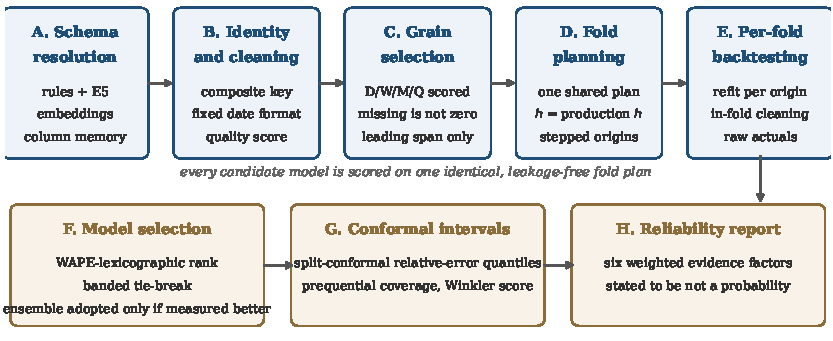
\includegraphics[width=\textwidth]{fig_architecture.pdf}
\caption{Pipeline architecture. Stages A--E prepare the series and produce
out-of-sample evidence; stages F--H convert that evidence into a forecast,
a calibrated-and-audited interval, and an explicit reliability statement.
Every candidate model is scored on one identical fold plan, which is what
makes the rankings in Section~\ref{sec:results} comparable.}
\label{fig:arch}
\end{figure*}

\subsection{Stage A: Semantic schema resolution}

Each column is described by its name, dtype, sample values, null count and
cardinality. A rule stage matches the normalised name against a synonym
dictionary of ERP naming conventions. A semantic stage expands ERP
abbreviations into words, appends detected value patterns, embeds the
resulting context with E5-large-v2~\cite{wang2022e5} and ranks it by cosine
similarity against pre-embedded canonical business names. The two stages are
combined: agreement raises confidence, disagreement retains the rule answer
and records the alternative. Human corrections are persisted to a JSON memory
consulted before either stage runs. If the embedding model is unavailable the
rule stage runs alone, which is the system's general degradation pattern.

\subsection{Stage B: Transaction identity and cleaning}

A repeated identifier is evidence that a column is not a primary key, not
evidence of duplication. The pipeline therefore resolves a \emph{composite
business key} --- invoice number, invoice date, product, customer, quantity and
net sales --- and only accepts it when at least three components
resolve \emph{and} the resolved set includes both a date and a measure; otherwise it degrades to
exact-row duplicate removal and reports the limitation. Rows identical on the
key are removed as re-imports; rows sharing an identifier but differing in
date, product, quantity or value are retained.

Dates are parsed deterministically: each candidate \texttt{strftime} format is
tried against the whole column, and the format that parses at least 80\% of
rows is applied to every row. This avoids per-row inference, under which
\texttt{06/04/23} may be resolved differently in different rows of the same
column. Row-level cleaning removes unparseable rows, implausible dates and
exact duplicates, and reports every count. A scalar data-quality score
$Q\in[0,1]$ penalises the fraction dropped, the fraction capped and the
missing-period ratio.

\subsection{Stage C: Forecast-grain selection}

Let $f\in\{\text{daily},\text{weekly},\text{monthly},\text{quarterly}\}$.
Transactions are summed into periods at $f$ over a gapless period index; a
period with no transaction is marked \emph{unobserved} rather than set to
zero, so an observed zero total and an absent record remain distinguishable.
Let $n_f$ be the number of periods, $o_f$ the number observed,
$d_f=o_f/n_f$ the density, $\mathrm{CV}_f$ the coefficient of variation and
$s_f$ an indicator that the series covers at least two full cycles of a
detectable seasonal period. A grain is rejected if $n_f<12$, if
$n_f<4h$, or if $d_f<0.60$. Surviving grains are scored
\begin{equation}
\begin{split}
G(f) = {}& 0.35\,d_f + 0.25\min\!\Big(1,\tfrac{n_f}{24}\Big)\\
        & + 0.15\max\!\Big(0,\,1-\min\big(1,\tfrac{\mathrm{CV}_f}{2}\big)\Big)\\
        & + 0.15\,s_f + 0.10\,\rho_f ,
\end{split}
\label{eq:grain}
\end{equation}
where $\rho_f\in\{1.0,0.75,0.50,0.25\}$ is a resolution preference from finest
to coarsest. The five terms encode: prefer a series that is measured rather
than filled; prefer more modelled periods, saturating at two annual cycles;
prefer lower dispersion; prefer a testable seasonal cycle; and, all else
equal, prefer the finer grain, which yields more validation origins and an
actionable resolution and can always be summed upward afterwards. The
resolution term is a deliberate counterweight: coarser aggregation
mechanically raises $d_f$ and lowers $\mathrm{CV}_f$, so a score built from
those two alone would drift to quarterly on almost any dataset.

Two properties keep this outside the evaluation loop. No model is fitted at
any point in~\eqref{eq:grain}, and the statistics that decide the winner are
computed on the leading 80\% of the calendar span, so the periods a later
walk-forward validation will score against cannot influence the choice. The
diagnostics reported to the user are computed on the full series, because
they describe the dataset rather than make the decision.

Missing periods are then filled by a strategy chosen from density alone: none
needed above 0.99; linear interpolation of runs of at most two unobserved
periods bounded by real activity above 0.75; zero-filling with an explicit
sparsity flag below that.

\subsection{Stage D: Shared fold planning}

One validation plan is derived per series and used by every candidate, so all
models are scored at identical origins. With $n$ periods, requested horizon
$h$ and seasonal period $m$, the first training window is
\begin{equation}
t_0=\max\big(8,\;2m,\;\lceil 0.5\,n\rceil\big),
\label{eq:mintrain}
\end{equation}
and the validation origins are
\begin{equation}
\mathcal{O}=\{\,t_0,\;t_0+\delta,\;\dots\le n-h\,\},\quad
\delta=\Big\lceil \tfrac{n-h-t_0+1}{12} \Big\rceil ,
\label{eq:origins}
\end{equation}
targeting about twelve origins spread across history rather than clustered at
one end. If fewer than three origins result, the seasonal requirement in
\eqref{eq:mintrain} is relaxed to $m$ and then to $0$; only if that still
fails is $h$ reduced, and the resulting mismatch between validation and
production horizon is recorded and reported rather than absorbed silently.

\subsection{Stage E: Per-fold backtesting}

For each origin $t\in\mathcal{O}$ and each candidate model $M$: outlier bounds
and gap bridging are fitted on the raw training prefix $y_{1:t}$ \emph{only};
$M$ is instantiated fresh and fitted on the transformed prefix; $h$ steps are
predicted; and the predictions are scored against \emph{raw} actuals
$y_{t+1:t+h}$, excluding any validation period that was never observed. Nothing
at or after $t$ participates in fitting either the model or the preprocessing,
so the protocol is leakage-free by construction rather than by
convention~\cite{kaufman2012leakage}. Fig.~\ref{fig:folds} shows the resulting
layout on the study dataset.

All folds' $(\text{actual},\text{predicted})$ pairs are pooled and each metric
computed once over the pooled arrays; averaging per-fold RMSEs would not be an
RMSE. The primary metric is
\begin{equation}
\mathrm{WAPE}=\frac{\sum_{i}\lvert y_i-\hat y_i\rvert}{\sum_{i}\lvert y_i\rvert}\times 100 ,
\label{eq:wape}
\end{equation}
a ratio of sums rather than a mean of per-point ratios, so a small number of
near-zero actuals cannot dominate
it~\cite{hyndman2006accuracy,davydenko2013measuring}. MAPE is computed only
over points with non-zero actuals, capped per point, reported as
informational, and never used to rank. Fold-to-fold consistency is summarised
as
\begin{equation}
S=1-\min\!\left(1,\;\frac{\sigma(\{w_k\})}{\mu(\{w_k\})}\right),
\label{eq:stability}
\end{equation}
where $w_k$ is fold $k$'s own WAPE; $S=1$ means identical error at every
origin.

\begin{figure}[!t]
\centering
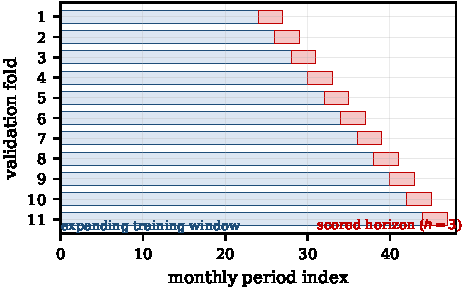
\includegraphics[width=\columnwidth]{fig_folds.pdf}
\caption{The shared walk-forward plan produced for the study dataset:
$n=48$ monthly periods, $t_0=24$, $\delta=2$, $h=3$, giving 11 folds and 33
scored points. Every candidate model is refitted from scratch on each blue
training window and scored on the adjacent red horizon.}
\label{fig:folds}
\end{figure}

\subsection{Stage F: Selection}

Models are ordered lexicographically by
$(\mathrm{WAPE},\mathrm{SMAPE},\mathrm{RMSE},\mathrm{MAE})$, with missing
metrics sorting last. Models whose primary metric lies within 5\% of the
leader's are treated as an empirical tie and reordered by a composite of
stability, simplicity, validated fold count and capability--series match; this
never reorders a model with a materially worse error ahead of a better one,
and the explanation states when it changed the pick.

Models within 25\% of the leader's error (at most four) form a candidate
ensemble weighted by inverse validation error, following Bates and
Granger~\cite{bates1969combination}:
\begin{equation}
\omega_j=\frac{1/e_j}{\sum_{l}1/e_l},\qquad
\hat y^{\text{ens}}_{t+i}=\sum_j \omega_j\,\hat y^{(j)}_{t+i}.
\label{eq:ensemble}
\end{equation}
Crucially, the blend is then \emph{re-scored} on the same folds as its
components, using weights derived at fold $k$ only from folds strictly before
$k$, and adopted only if its measured WAPE improves on the best single model
by at least 1\%. When it is adopted, the metrics reported are the ensemble's
own; when it is rejected, the measurement is still reported.

\subsection{Stage G: Conformal prediction intervals}

For each retained fold pair the relative error
$r=(y-\hat y)/\hat y$ is collected. Because actuals are non-negative and
predictions positive, $r\ge-1$, so a lower bound built from $r$ cannot become
negative --- a property of the construction, not a clip. For $N$ errors and
level $1-\alpha$, the split-conformal order statistics are indexed by
\begin{equation}
k_{\text{lo}}=\Big\lfloor (N{+}1)\tfrac{\alpha}{2}\Big\rfloor,\qquad
k_{\text{hi}}=\Big\lceil (N{+}1)\big(1-\tfrac{\alpha}{2}\big)\Big\rceil ,
\label{eq:conformal}
\end{equation}
and the interval for a point forecast $\hat y$ is
$\big[\hat y(1+r_{(k_{\text{lo}})}),\,\hat y(1+r_{(k_{\text{hi}})})\big]$.
When $k_{\text{hi}}>N$ the level is not attainable from $N$ errors ---
two-sided 95\% requires $N\ge39$ --- and the bound is labelled
\textsc{extrapolated} rather than presented as a guarantee. Errors are pooled
across horizon steps unless every step has enough of its own errors for the
tightest level to be an interior order statistic, in which case horizon-specific
quantiles are used; the choice and its consequence are stated in the output.

Coverage is measured \emph{prequentially}: the interval tested at fold $k$ is
built only from folds strictly before $k$, so the coverage figure is itself
out-of-sample. Sharpness is measured by the Winkler
score~\cite{winkler1972interval}
\begin{equation}
W_\alpha=(u-l)+\frac{2}{\alpha}(l-y)\mathbf{1}[y<l]+\frac{2}{\alpha}(y-u)\mathbf{1}[y>u],
\label{eq:winkler}
\end{equation}
a proper scoring rule~\cite{gneiting2007scoring} that charges for width, so
coverage cannot be bought by widening alone.

\subsection{Stage H: Reliability reporting}

A weighted composite over six measured factors --- accuracy, fold-to-fold
consistency, history, input quality, interval calibration and selection
margin,
\begin{equation}
R=\textstyle\sum_{j} \lambda_j\,\phi_j,\quad
\boldsymbol{\lambda}=(0.28,0.22,0.18,0.12,0.12,0.08),
\label{eq:reliability}
\end{equation}
--- is mapped to a level (\textsc{high} $\ge0.70$, \textsc{moderate}
$\ge0.50$, \textsc{low} $\ge0.30$, else \textsc{very low}) and returned with a
per-factor breakdown. Each $\phi_j$ is anchored to a meaningful reference:
accuracy against 100\% WAPE, the score obtained by forecasting zero
everywhere; selection margin against the fold-to-fold standard deviation, so a
winning margin smaller than the noise is not counted as evidence. Interval
width is reported but deliberately \emph{not} scored, since it is a function
of the error distribution that accuracy and consistency already measure. The
output states in text that $R$ is an evidence rating and not a probability
that the forecast is correct.

% ===========================================================================
\section{Experimental Setup}
\label{sec:setup}

\subsection{Dataset}

The study dataset is the ERP export bundled with the system: a four-year
invoice-level extract summarised in Table~\ref{tab:dataset}. It is
representative of the target setting --- a single mid-sized organisation with a
few hundred invoices per year across a handful of regions, product groups and
customer segments --- and it exhibits the specific pathologies the pipeline is
designed to handle: abbreviated column names, missing values in four business
fields, and invoice numbers that repeat across genuinely different
transactions.

\begin{table}[!t]
\caption{Study dataset characteristics.}
\label{tab:dataset}
\centering
\footnotesize
\begin{tabular}{@{}ll@{}}
\toprule
Property & Value \\
\midrule
Records (invoice line rows)      & 392 \\
Columns                          & 21 \\
Date range                       & 2021-01-03 to 2024-12-27 \\
Calendar span                    & 1{,}454 days \\
Total net sales                  & 59{,}203{,}948.47 INR \\
Distinct customers / products    & 30 / 15 \\
Regions / product groups         & 4 / 5 \\
Salespeople / customer segments  & 5 / 3 \\
Missing values                   & \texttt{cust\_nm} 17, \texttt{nsv} 8, \\
                                 & \texttt{mrgn\_pct} 13, \texttt{dlv\_st} 10 \\
Distinct invoice numbers         & 180 (212 rows share one) \\
Monthly periods (observed)       & 48 of 48 \\
Monthly coefficient of variation & 0.6087 \\
\bottomrule
\end{tabular}
\end{table}

\subsection{Models and configuration}

Nine forecasters are available: Naive, Seasonal Naive, Moving Average, Simple
Exponential Smoothing (SES), Holt's linear trend, Holt--Winters and SARIMA
(\texttt{statsmodels}), Prophet~\cite{taylor2018prophet}, and
XGBoost~\cite{chen2016xgboost} over lag, rolling, trend and calendar features.
The ablation study additionally instantiates Ridge, ElasticNet, Random Forest
and Gradient Boosting over the same feature families through a common tabular
wrapper, so that feature set and estimator can be varied independently.
Hyperparameters, where a model exposes any, are tuned once per run on the
first fold's training prefix and then held fixed across all folds and the
final fit, so reported accuracy describes the configuration that produces the
forecast.

\subsection{Protocol}

Unless stated otherwise, all results use the shared plan of
\eqref{eq:mintrain}--\eqref{eq:origins} at $h=3$: $t_0=24$, $\delta=2$,
11 folds, 33 scored points. All experiments were run on Python 3.11 with
pandas 2.2.0, NumPy 1.26.4, scikit-learn 1.4.2, statsmodels 0.14.2, XGBoost
2.1.1 and \texttt{sentence-transformers} 2.7.0 on Windows 11, single machine,
candidate training executed sequentially.

Prophet was installed but its compiled Stan backend was non-functional in this
environment; every Prophet fit raised inside its isolated subprocess. This is
reported rather than hidden because it exercises the fault-isolation path: the
pipeline recorded the failure, excluded Prophet from the ranking and completed
normally. Prophet results are consequently absent from all tables, and no
claim is made about its accuracy here.

\subsection{Experiments}

\begin{itemize}
\item[E1] \emph{Schema and identity.} Column mapping from a cold start (no
      persisted memory); business-key resolution against naive
      single-identifier deduplication.
\item[E2] \emph{Grain.} Structural diagnostics for all four candidate grains,
      plus the best achievable error at each usable grain under an identical
      protocol.
\item[E3] \emph{Model comparison.} All available models under the shared plan,
      with and without one-shot hyperparameter tuning, plus the measured
      ensemble.
\item[E4] \emph{Protocol.} Single trailing hold-out versus walk-forward at
      $h=1$ and $h=3$, compared by error and by rank agreement.
\item[E5] \emph{Leakage.} Preprocessing fitted on the whole series before
      splitting versus refitted inside each fold.
\item[E6] \emph{Metric behaviour.} An $\varepsilon$-guarded MAPE against the
      pipeline's zero-excluded MAPE and WAPE on a sparse grain.
\item[E7] \emph{Features.} A controlled ablation ladder over lag, rolling,
      trend and calendar families across five estimators, with in-sample error
      recorded alongside validation error.
\item[E8] \emph{Uncertainty and reliability.} Prequential coverage, sharpness
      and the reliability decomposition for the published forecast.
\item[E9] \emph{Segments.} The full pipeline applied independently to every
      value of three business dimensions.
\end{itemize}

% ===========================================================================
\section{Results and Analysis}
\label{sec:results}

\subsection{Schema resolution and transaction identity (E1)}

From a cold start the two-stage mapper resolved all 21 columns to the correct
business concept, verified by manual inspection against the column semantics,
with mean confidence 0.943 and every column above the 0.75 high-confidence
threshold; the cold run took 31.6~s including embedding-model load. The two
stages agreed on 13 of 21 columns. On the remaining 8 the embedding stage's
top suggestion differed from the rule match --- proposing, for example,
\emph{customer code} for \texttt{cust\_nm} and \emph{quantity sold} for
\texttt{slsp} --- and in all 8 cases the retained rule answer was the correct
one. On this schema the semantic stage therefore contributed confirmation and
alternatives rather than corrections; with only 21 columns this is an
observation about one ERP vocabulary, not a general claim about embedding-based
matching.

Transaction identity produced the study's sharpest data-preparation result.
The composite key \texttt{inv\_no + inv\_dt + prod\_id + cust\_cd + qty\_sold
+ nsv} resolved fully. It identified 7 exact duplicate rows and 20 business-key
duplicates, removing 20 rows (5.1\%) and retaining 372. Of the 212 rows that
share an invoice number with another row, 192 were preserved as distinct
transactions. Deduplicating on the invoice-number column alone --- the natural
choice if a repeated identifier is read as duplication --- would have reduced
the dataset from 392 rows to 180 ($-54.08\%$) and destroyed 56.65\% of total
recorded revenue, leaving every downstream forecast fitted on less than half
the history.

\subsection{Forecast-grain selection (E2)}

Inter-arrival inference on this dataset returns \emph{weekly}: invoices arrive
roughly every four days. Table~\ref{tab:grain} and Fig.~\ref{fig:grain} show
what the four candidate grains actually look like.

\begin{table}[!t]
\caption{Candidate forecast grains. Score is~\eqref{eq:grain} computed on the
leading 80\% of the calendar span; best WAPE is the lowest achieved by any of
the eight available models under an identical $h=3$ plan at that grain.}
\label{tab:grain}
\centering
\footnotesize
\setlength{\tabcolsep}{4pt}
\begin{tabular}{@{}lrrrrrr@{}}
\toprule
Grain & Periods & Density & CV & Score & Folds & Best \\
      &         & (\%)    &    &       &       & WAPE (\%) \\
\midrule
Daily     & 1{,}455 & 22.7  & 3.936 & --- (rej.) & --- & --- \\
Weekly    & 209     & 84.7  & 1.231 & 0.7602 & 12 & 69.03 \\
\textbf{Monthly} & \textbf{48} & \textbf{100.0} & \textbf{0.609} & \textbf{0.8691} & \textbf{11} & \textbf{47.48} \\
Quarterly & 16      & 100.0 & 0.316 & 0.8019 & 6  & 12.87 \\
\bottomrule
\end{tabular}
\end{table}

\begin{figure*}[!t]
\centering
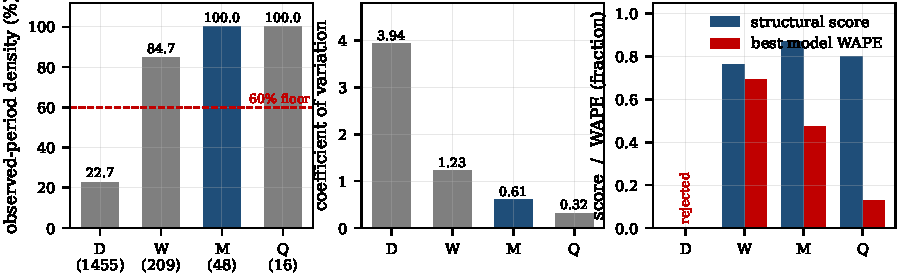
\includegraphics[width=\textwidth]{fig_grain.pdf}
\caption{Grain diagnostics. Left: observed-period density; the daily grain
falls below the 60\% floor and is rejected. Centre: coefficient of variation.
Right: structural score~\eqref{eq:grain} against the best model WAPE actually
achieved at that grain. Density and dispersion improve monotonically with
coarser aggregation, which is why the score includes an explicit resolution
counterweight.}
\label{fig:grain}
\end{figure*}

The daily grain is rejected: only 22.7\% of days contain a transaction, so
77.3\% of the modelled series would be fill rather than measurement. The
weekly grain that inter-arrival inference implies is usable but poor: 32 of
209 weeks are unobserved and the coefficient of variation is 1.231, double
the monthly value. The selected monthly grain is fully observed. The accuracy
consequence is large: the best of eight models achieves 47.48\% WAPE at
monthly grain against 69.03\% at weekly --- a 21.55~pp difference produced
by a decision taken before any model was fitted. It is worth stating that
these two numbers are not measurements of the same quantity, since a weekly
error and a monthly error are relative to differently aggregated targets; the
comparison is nonetheless the operative one, because the system must publish a
forecast at one of them.

Quarterly grain achieves a still lower 12.87\% WAPE, and the pipeline does not
select it. This is a deliberate trade-off encoded in the resolution term of
\eqref{eq:grain}: quarterly leaves only 16 periods and 6 validation origins,
and a quarterly forecast is far less actionable than a monthly one. The
mechanism is transparent --- aggregation averages away noise, which lowers
relative error at every grain --- and it is the reason \eqref{eq:grain} is not
simply ``minimise WAPE over grains''. We return to this in
Section~\ref{sec:discussion}.

Grain choice also changes how the series is characterised. Computed on raw
transaction rows, the series has $\mathrm{CV}=1.7242$ and classifies as
\emph{Highly Volatile} (confidence 0.93), which routes candidate selection
toward XGBoost, Prophet and SARIMA. Computed on the modelled monthly series it
has $\mathrm{CV}=0.6087$ and classifies as \emph{Long History}, routing toward
SARIMA and Prophet. The first characterisation describes invoice-to-invoice
spread, which no model in this pipeline is ever asked to predict.

\subsection{Model comparison (E3)}

Table~\ref{tab:models} and Fig.~\ref{fig:models} give the full comparison
under the shared 11-fold plan, ranked by the pooled WAPE of~\eqref{eq:wape}.

\begin{table}[!t]
\caption{All available models under one identical plan (monthly grain, $h=3$,
11 folds, 33 scored points). $S$ is fold-to-fold stability~\eqref{eq:stability}.
Runtime is total fit-and-predict time across all folds.}
\label{tab:models}
\centering
\footnotesize
\setlength{\tabcolsep}{3.5pt}
\begin{tabular}{@{}lrrrrrr@{}}
\toprule
Model & WAPE & SMAPE & MAE & RMSE & $S$ & Time \\
      & (\%) & (\%)  & (kINR) & (kINR) &  & (s) \\
\midrule
\textbf{SES}            & \textbf{47.48} & 46.90 & 657 & 871 & 0.602 & 0.00 \\
Naive                   & 51.80 & 49.55 & 717 & 1007 & 0.534 & 0.00 \\
Holt linear             & 53.27 & 52.19 & 738 & 950  & 0.585 & 0.01 \\
Moving average          & 54.59 & 52.56 & 756 & 975  & 0.373 & 0.00 \\
Holt--Winters           & 57.56 & 54.83 & 797 & 1033 & 0.451 & 0.53 \\
XGBoost                 & 62.44 & 58.80 & 864 & 1072 & 0.132 & 1.25 \\
Seasonal naive          & 63.89 & 63.98 & 885 & 1183 & 0.420 & 0.01 \\
SARIMA                  & 67.66 & 66.71 & 937 & 1132 & 0.469 & 1.08 \\
\midrule
Ensemble (SES+Naive+Holt) & 50.05 & 49.08 & 693 & 913 & --- & --- \\
\bottomrule
\end{tabular}
\end{table}

\begin{figure}[!t]
\centering
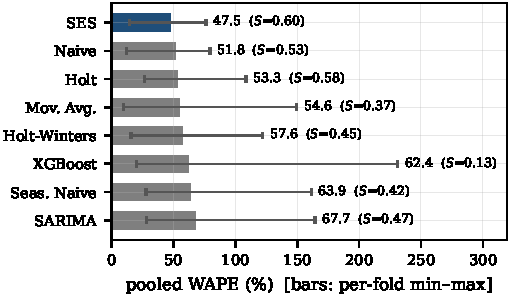
\includegraphics[width=\columnwidth]{fig_models.pdf}
\caption{Pooled WAPE by model at monthly grain, with whiskers spanning the
per-fold minimum and maximum and $S$ the stability
score~\eqref{eq:stability}. The spread within a model is comparable to the
spread between models, which is the basis for the selection-margin factor in
\eqref{eq:reliability}.}
\label{fig:models}
\end{figure}

The ordering is unambiguous and consistent with the large-scale
evidence~\cite{makridakis2018statml,spiliotis2022sku}: the three lowest-error
models are the three simplest. SES leads at 47.48\% WAPE; SARIMA, with the
most parameters to estimate from 24--45 training points, is last at 67.66\%;
XGBoost is sixth at 62.44\% with by far the worst stability ($S=0.132$). The
three-model inverse-error ensemble of~\eqref{eq:ensemble} was constructed,
scored on the same folds, measured at 50.05\% --- worse than SES --- and
rejected, with the measurement reported. Selection is thus decided by evidence, not by a prior that blends
are better.

One-shot hyperparameter tuning on the first fold's prefix helped one model and
hurt two: Holt--Winters improved from 57.56\% to 56.43\%, while SARIMA
degraded from 67.66\% to 73.70\% and XGBoost from 62.44\% to 63.65\%. The
remaining models either self-tune inside \texttt{fit} or have nothing to tune.
Tuning a multi-parameter model on the earliest, shortest window and holding
that choice fixed is evidently not reliably beneficial at this sample size.

Wall-clock cost is dominated by failure handling rather than by fitting: the
eight successful models consume 2.9~s of fit-and-predict time in total, while
the full benchmark takes 133.9~s, almost all of it spent starting and reaping
isolated subprocesses for the 11 Prophet folds that could not run in this
environment.

\subsection{Validation protocol (E4)}

Table~\ref{tab:protocol} and Fig.~\ref{fig:protocol} compare three protocols
on the same series and the same models.

\begin{table}[!t]
\caption{Effect of the validation protocol. Rank correlations are against the
walk-forward $h=3$ ordering over the eight models.}
\label{tab:protocol}
\centering
\footnotesize
\setlength{\tabcolsep}{3.5pt}
\begin{tabular}{@{}lccccc@{}}
\toprule
Protocol & Origins & Points & Best model & WAPE & $\rho$ \\
\midrule
Single hold-out, $h{=}3$ & 1  & 3  & Seasonal naive & 11.52 & $-0.381$ \\
Walk-forward, $h{=}1$    & 12 & 12 & SES            & 55.30 & $\phantom{-}0.738$ \\
Walk-forward, $h{=}3$    & 11 & 33 & SES            & 47.48 & --- \\
\bottomrule
\end{tabular}
\end{table}

\begin{figure*}[!t]
\centering
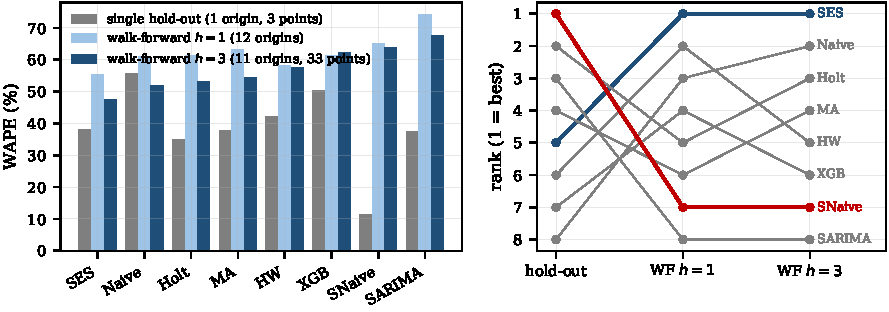
\includegraphics[width=\textwidth]{fig_protocol.pdf}
\caption{Left: per-model WAPE under three validation protocols. Right: rank
migration. Seasonal naive (red) is ranked best by a single trailing hold-out
and seventh of eight by walk-forward validation at the same horizon; SES
(blue) moves in the opposite direction.}
\label{fig:protocol}
\end{figure*}

The single trailing hold-out --- one origin, three scored points, the
configuration a naive train/test split produces --- reports 11.52\% WAPE for
seasonal naive, which walk-forward validation at the same horizon places
seventh of eight at 63.89\%. It also reports 38.08\% for SES, which is 9.4~pp
better than the value 33 out-of-sample points support. The rank correlation
between the two orderings is $\rho=-0.381$ ($p=0.352$; Kendall
$\tau=-0.214$, $p=0.548$): with eight models the hold-out ordering is
statistically indistinguishable from an arbitrary one. By contrast, the two
multi-origin protocols agree substantially ($\rho=0.738$, $p=0.037$; Kendall
$\tau=0.643$, $p=0.031$) and select the same winner, so the disagreement is
attributable to the number of origins rather than to the horizon.

This is a concrete, quantified instance of what Tashman~\cite{tashman2000outofsample}
and Bergmeir and Ben\'itez~\cite{bergmeir2012cv} argue in general. Its
practical weight is high: a system that reports 11.52\% WAPE for a model whose
honest error is 63.89\% is not slightly optimistic, it is recommending the
wrong model with a fabricated justification.

\subsection{Preprocessing leakage (E5)}

Table~\ref{tab:leakage} isolates the cost of fitting preprocessing before
splitting rather than inside each fold.

\begin{table}[!t]
\caption{Optimism from whole-series preprocessing. $\Delta$ is the honest
(per-fold) WAPE minus the leaky (whole-series) WAPE, in percentage points;
positive means the leaky protocol reported a better result than the model
deserves.}
\label{tab:leakage}
\centering
\footnotesize
\setlength{\tabcolsep}{3pt}
\begin{tabular}{@{}lrrrrr@{}}
\toprule
& \multicolumn{3}{c}{Weekly grain, $3.0\times$IQR} & \multicolumn{2}{c}{Monthly, $1.5\times$IQR} \\
\cmidrule(lr){2-4}\cmidrule(lr){5-6}
Model & Honest & Leaky & $\Delta$ & Honest & $\Delta$ \\
\midrule
SES            & 69.03 & 62.75 & $+6.28$ & 47.48 & $+1.59$ \\
Naive          & 85.51 & 82.60 & $+2.91$ & 51.80 & $+0.99$ \\
Moving average & 81.00 & 77.19 & $+3.81$ & 54.59 & $+1.96$ \\
Holt linear    & 75.69 & 70.87 & $+4.82$ & 53.27 & $+2.11$ \\
Seasonal naive & 82.33 & 78.78 & $+3.55$ & 63.89 & $+2.80$ \\
Holt--Winters  & 72.64 & 68.21 & $+4.43$ & 57.56 & $+1.08$ \\
SARIMA         & 77.66 & 73.98 & $+3.68$ & 67.66 & $+2.37$ \\
XGBoost        & 82.55 & 77.60 & $+4.95$ & 62.44 & $+15.63$ \\
\midrule
Mean           &       &       & $+4.30$ &       & $+3.57$ \\
\bottomrule
\end{tabular}
\end{table}

At the deployed setting --- monthly grain, $3.0\times$IQR capping --- no period
in this series exceeds the bound and no period is unobserved, so the guard is
inert and $\Delta=0.00$ for every model. That is an honest null result and it
is worth stating plainly: on this dataset the leakage-free construction costs
nothing and gains nothing.

The guard becomes measurable as soon as preprocessing is active. On the weekly
grain, where 32 periods are unobserved and 15 periods exceed the whole-series
IQR bound, whole-series preprocessing understates error by 2.91--6.28~pp
(mean 4.30~pp) across all eight models. On the monthly grain with the
multiplier tightened to $1.5\times$ so that two periods are capped --- a
sensitivity analysis, not the deployed configuration --- the classical models
gain 0.99--2.80~pp of unearned accuracy while XGBoost gains 15.63~pp, falling
from 62.44\% to 46.81\%: it rises from sixth place to second and its gap to
SES narrows from 14.96~pp to 0.92~pp. The model most able to exploit
information about the periods it is about to be scored on benefits most from
being given it, which is precisely the mechanism Kaufman
\emph{et al.}~\cite{kaufman2012leakage} describe.

\subsection{Error-measure behaviour (E6)}

On the daily grain (1{,}455 periods, 77.7\% of them zero) an
$\varepsilon$-guarded MAPE with $\varepsilon=10^{-9}$ --- the defensive
formulation a system might adopt to avoid a division-by-zero crash --- returns
$6.36\times10^{14}\%$ for moving average and $4.25\times10^{14}\%$ for SES,
while the same forecasts score 93.79\% and 100.11\% under the pipeline's
zero-excluded MAPE and 97.46\% and 96.74\% under WAPE (12 folds, 10 scored
points, one of which has a zero actual). A single zero actual
divided by $\varepsilon$ is enough to make the average meaningless without
producing an error, and any ranking that consulted it would be decided by the
denominator rather than the model. This is the concrete form of the concerns
raised in~\cite{hyndman2006accuracy,davydenko2013measuring,kolassa2020bestpoint}
and the reason MAPE is excluded from every ranking decision in
Section~\ref{sec:method}.

\subsection{Feature engineering (E7)}

Table~\ref{tab:ablation} and Fig.~\ref{fig:ablation} report the controlled
ablation: identical fold plan, identical preprocessing, one feature family or
estimator varied at a time.

\begin{table}[!t]
\caption{Feature ablation, monthly grain, 11 folds. Train is in-sample WAPE on
the last fold's training window; O/F is validation/train error. Verdict uses a
1~pp separability threshold against the SES baseline. Selected rows; 22
configurations were evaluated in total (15 machine-learning, 7 univariate
statistical), and none was accepted.}
\label{tab:ablation}
\centering
\footnotesize
\setlength{\tabcolsep}{3pt}
\begin{tabular}{@{}llrrrl@{}}
\toprule
Configuration & Features & WAPE & Train & O/F & Verdict \\
              &          & (\%) & (\%)  &     & \\
\midrule
SES (baseline)      & none        & 47.48 & 48.21 & 0.98 & baseline \\
Random forest       & lag+roll    & 47.64 & 24.84 & 1.92 & rejected \\
Ridge               & trend       & 47.78 & 41.10 & 1.16 & rejected \\
Ridge               & calendar    & 50.04 & 45.82 & 1.09 & rejected \\
XGBoost             & lag+roll    & 50.55 & 13.10 & 3.86 & rejected \\
XGBoost             & rolling     & 50.67 & 24.19 & 2.09 & rejected \\
Gradient boosting   & lag+roll    & 51.86 & \phantom{0}9.12 & 5.69 & rejected \\
XGBoost             & all         & 53.16 & 11.16 & 4.76 & rejected \\
XGBoost             & lags        & 56.01 & 16.69 & 3.36 & rejected \\
ElasticNet          & lag+roll    & 67.42 & 41.85 & 1.61 & rejected \\
Ridge               & all         & 84.93 & 32.45 & 2.62 & rejected \\
\bottomrule
\end{tabular}
\end{table}

\begin{figure}[!t]
\centering
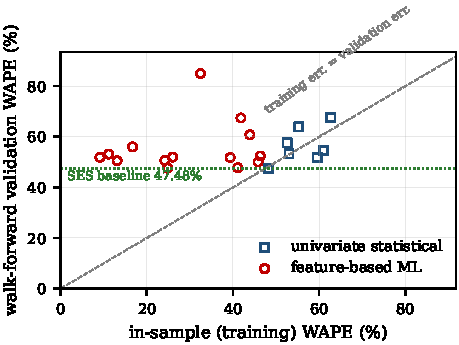
\includegraphics[width=\columnwidth]{fig_ablation.pdf}
\caption{In-sample against walk-forward validation error for every ablation
configuration. Univariate statistical methods sit close to the diagonal;
feature-based learners sit far above it, achieving low training error and no
validation benefit.}
\label{fig:ablation}
\end{figure}

No configuration reached the 1~pp improvement threshold; the closest, a random
forest on lag and rolling features, was 0.16~pp \emph{worse} than SES. The
in-sample column explains why. Gradient boosting reaches 9.12\% training WAPE
and validates at 51.86\% ($5.69\times$); XGBoost on lags and rolling features
reaches 13.10\% and validates at 50.55\% ($3.86\times$). SES, by contrast, has
a ratio of 0.98 --- its in-sample and out-of-sample errors are the same, which
is what a two-parameter model on 24--45 points should look like. Combining every
family together did not help either: XGBoost over all 18 selected features
scored 53.16\%, worse than XGBoost over lags and rolling alone (50.55\%), and
Ridge over all families reached 84.93\%, its worst configuration by a wide
margin. With at most 45 training rows, the
binding constraint is sample size, not feature availability.

\subsection{Uncertainty and reliability (E8)}

Fig.~\ref{fig:forecast} shows the published forecast and its intervals, and
Table~\ref{tab:intervals} the calibration audit.

\begin{figure*}[!t]
\centering
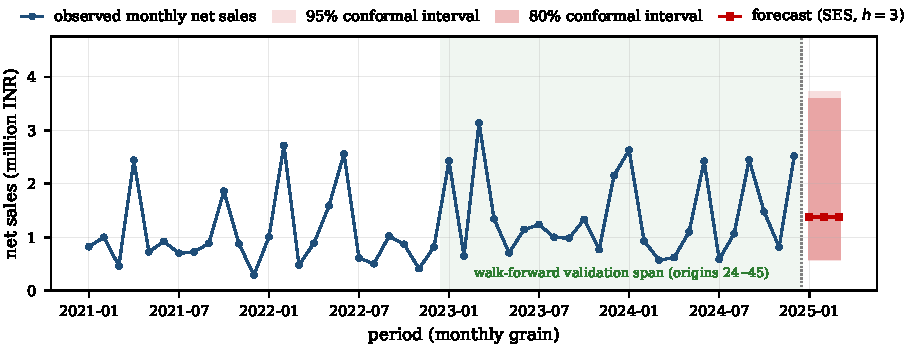
\includegraphics[width=\textwidth]{fig_forecast.pdf}
\caption{Monthly net sales, the selected model's three-period forecast and its
split-conformal intervals. The point forecast is flat because SES was
selected; the interval width, not the point path, carries the uncertainty.}
\label{fig:forecast}
\end{figure*}

\begin{table}[!t]
\caption{Prediction interval audit for the published company forecast.
Coverage is prequential over 21 out-of-sample points; width is normalised by
the point forecast; the Winkler score~\eqref{eq:winkler} is in million INR.}
\label{tab:intervals}
\centering
\footnotesize
\begin{tabular}{@{}lrr@{}}
\toprule
Quantity & 80\% level & 95\% level \\
\midrule
Nominal coverage (\%)          & 80.0 & 95.0 \\
Observed coverage (\%)         & 66.7 & 66.7 \\
Coverage error (pp)            & $-13.3$ & $-28.3$ \\
Binomial standard error (pp)   & 10.3 & 10.3 \\
Mean normalised width          & 2.255 & 2.327 \\
Winkler score (MINR)           & 2.839 & 3.305 \\
Estimator status               & conformal & extrapolated \\
\bottomrule
\end{tabular}
\end{table}

\begin{figure}[!t]
\centering
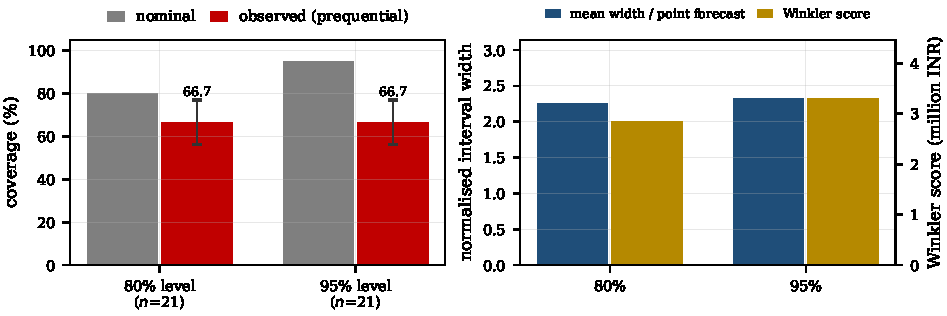
\includegraphics[width=\columnwidth]{fig_intervals.pdf}
\caption{Left: nominal against prequentially measured coverage, with binomial
standard errors. Right: sharpness. Both levels under-cover; the 95\% level
additionally exceeds what 33 errors can support as a conformal guarantee and
is labelled \textsc{extrapolated}.}
\label{fig:intervals}
\end{figure}

The 11 folds yield 33 relative errors, 11 per horizon step. That is below the
19 per step needed for an 80\% quantile to be an interior order statistic, so
the system pools across horizons and says so; it is also below the 39 needed
for a two-sided 95\% conformal interval, so $k_{\text{hi}}>N$ in
\eqref{eq:conformal} and the 95\% level is labelled \textsc{extrapolated}.
Measured prequentially, the 80\% interval contained the outcome 66.7\% of the
time over 21 points ($-13.3$~pp, standard error 10.3~pp) and the 95\% interval
likewise 66.7\% ($-28.3$~pp); Fig.~\ref{fig:intervals} plots both against
nominal alongside the corresponding sharpness. The intervals under-cover, and
the system reports this rather than presenting the nominal levels as
achieved. The Winkler score rises from 2.839 to 3.305 MINR between
the levels, confirming that the wider band is not simply better.

The reliability composite~\eqref{eq:reliability} returns $R=0.602$
(\textsc{moderate}) with the decomposition in Table~\ref{tab:reliability}. Two
factors are explicitly negative --- interval calibration (0.167) and selection
strength (0.267) --- and both correspond to real weaknesses established above:
the intervals under-cover, and SES's 4.58~pp margin over naive is only
$0.27\times$ the 17.15~pp fold-to-fold standard deviation, so the ranking
could plausibly change on different data. The legacy scalar confidence for the
same forecast is 65\%, which conveys none of this.

\begin{table}[!t]
\caption{Reliability decomposition for the published company forecast,
$R=0.602$ (\textsc{moderate}).}
\label{tab:reliability}
\centering
\footnotesize
\begin{tabular}{@{}llrr@{}}
\toprule
Factor & Measured value & $\phi_j$ & $\lambda_j$ \\
\midrule
Accuracy              & WAPE 46.82\%                   & 0.532 & 0.28 \\
Consistency           & fold s.d.\ 17.15 over 11 folds & 0.622 & 0.22 \\
History               & 48 periods, 11 folds           & 0.889 & 0.18 \\
Input data quality    & 100\% observed, $Q=0.91$       & 0.957 & 0.12 \\
Interval calibration  & 80\% level covers 66.7\%       & 0.167 & 0.12 \\
Selection strength    & $+4.58$ pp over naive          & 0.267 & 0.08 \\
\bottomrule
\end{tabular}
\end{table}

The published forecast itself is SES-selected at 46.82\% WAPE, with all three
periods at 1.378~MINR, an 80\% interval of [0.598, 3.575]~MINR and a
data-quality score of 0.913. It differs slightly from the 47.48\% benchmark
figure of Table~\ref{tab:models} because the production path applies row-level
cleaning before aggregation, removing 17 rows that duplicate another row on
the (date, value) pair --- a looser criterion than the six-column business key
of Section~\ref{sec:results}-A, which removed 20 rows on the full record.

\subsection{Segment-level forecasting (E9)}

Nine of the 21 columns qualified as business dimensions under the cardinality,
missingness and uniqueness safeguards; invoice number, at 180 distinct values,
was correctly excluded as an identifier. Table~\ref{tab:segments} reports the
full pipeline run independently for every value of three of them.

\begin{table}[!t]
\caption{Independent pipeline runs per business segment. Grain, model,
intervals and reliability are all resolved separately for each segment.}
\label{tab:segments}
\centering
\footnotesize
\setlength{\tabcolsep}{3pt}
\begin{tabular}{@{}llrrlrr@{}}
\toprule
Dimension & Value & Rows & Per. & Selected model & WAPE & Cov.\\
          &       &      &      &                & (\%) & 80 (\%)\\
\midrule
Region & North       & 89  & 48 & SES              & 50.43 & 88.2 \\
Region & East        & 92  & 46 & Ensemble (2)     & 57.48 & 83.3 \\
Region & West        & 121 & 48 & Moving average   & 65.14 & 78.9 \\
Region & South       & 90  & 48 & Naive            & 76.27 & 86.7 \\
Product & Automotive & 45  & 16 & SES              & 56.67 & 80.0 \\
Product & Electronics& 70  & 16 & SES              & 58.53 & 83.3 \\
Product & Industrial & 71  & 48 & Moving average   & 75.77 & 80.0 \\
Product & FMCG       & 103 & 48 & Ensemble (4)     & 77.48 & 85.0 \\
Product & Healthcare & 103 & 48 & SES              & 80.35 & 72.2 \\
Segment & Enterprise & 126 & 48 & Moving average   & 57.32 & 76.2 \\
Segment & Government & 143 & 48 & SES              & 57.61 & 95.0 \\
Segment & SMB        & 123 & 48 & SES              & 73.99 & 88.2 \\
\bottomrule
\end{tabular}
\end{table}

All twelve segments were classified as having sufficient history for
validation. Errors span 50.43--80.35\% WAPE, uniformly worse than the 46.82\%
company figure, as expected when the same total demand is split into thinner
series. Model choice varies by segment --- SES six times, moving average three,
naive once, an adopted ensemble twice --- confirming that per-segment selection
is doing work rather than reproducing one global answer. Two product groups
(Automotive, Electronics) had their grain resolved to quarterly rather than
monthly, because at monthly grain their transactions do not fill enough
periods; grain selection is therefore also per-segment, not inherited from the
company run. Reliability levels distribute as seven \textsc{moderate}, four
\textsc{low} and one \textsc{very low}, and interval coverage at the 80\% level
ranges from 72.2\% to 95.0\%, i.e.\ segment intervals are closer to nominal
than the company interval, though each rests on a comparably small number of
out-of-sample points.

% ===========================================================================
\section{Discussion}
\label{sec:discussion}

\subsection{The decisions before the model dominate}

Ordering the effects measured above by magnitude gives a clear picture. Record
identity, if resolved by the obvious wrong rule, removes 54\% of the data.
Grain choice moves best achievable error by 21.55~pp. Evaluation protocol
changes the headline error by 35.96~pp (11.52\% against 47.48\%), understates
its own chosen model's error by 52.37~pp, and inverts the ranking. Preprocessing placement moves error by up to 15.63~pp for the most
flexible model. Against these, the spread across all eight forecasting models
under the correct protocol is 20.18~pp, and the spread across the top three is
5.79~pp. On a series of this length the pre-model decisions are not
preliminaries to the modelling problem; several of them are larger than it.

This reframes what an automated forecasting system for enterprise data should
automate. The value is not primarily in searching a model space --- the
evidence from M-competition-scale
studies~\cite{makridakis2018statml,makridakis2022m5acc,spiliotis2022sku} and
from our own ablation is that the search converges on a simple method anyway
--- but in making the preparatory decisions defensibly and reporting what they
cost.

\subsection{Why simple methods win here, and what would change that}

SES beating SARIMA by 20.18~pp and XGBoost by 14.96~pp is not a surprising
result, and we do not present it as one. With 24--45 training points, SARIMA
must estimate autoregressive, differencing and moving-average orders and
XGBoost must learn splits over up to 18 features. The ablation makes the
mechanism visible: the tree models reach single-digit in-sample error and gain
nothing out of sample. The overfitting ratio, reported alongside every
configuration, is what turns this from an assertion into a measurement.

The conditions under which this would change are identifiable. Cross-series
learning over many products would give tree and neural models the sample size
they lack~\cite{monteromanso2020fforma,shchur2023autogluon}; genuinely
exogenous, forecast-time-available drivers (price plans, promotions,
committed pipeline) would give them information the target's own past does not
contain. The pipeline's availability contract makes the second point
enforceable: it classifies every mapped column by whether its future value is
knowable at forecast time, and on this export no column qualified. The four
columns most correlated with net sales are arithmetic restatements of it, and
the rest are business outcomes whose future values would themselves have to be
forecast.

\subsection{The grain trade-off is a choice, and it is visible}

Quarterly aggregation achieves 12.87\% WAPE against monthly's 47.48\%, and the
system selects monthly. This is the least comfortable result in the paper and
we state it as a design decision rather than an optimum. Relative error falls
mechanically with aggregation because averaging cancels noise, so an
error-minimising grain selector would drive every dataset to its coarsest
admissible level. Monthly is chosen because it yields 48 modelled periods
against 16, 11 validation origins against 6, and a forecast at a resolution a
business can plan against. The resolution weight in~\eqref{eq:grain} is
0.10 --- small, but the term exists precisely so this pull is explicit rather
than emergent. A deployment that genuinely wants quarterly planning can raise
it; what the system will not do is silently choose the coarsest grain and
present the resulting low error as skill. Temporal
hierarchies~\cite{athanasopoulos2017temporal} offer a principled alternative
we did not implement: forecast at several levels and reconcile.

\subsection{Reporting calibration failure is a feature}

The published 80\% interval covers 66.7\% of outcomes. A system could avoid
this number in three ways: not measure coverage, measure it in-sample on the
errors the quantile was fitted to, or widen the band until coverage is
attained. The first two are the common cases; the third is defeated by the
Winkler score, which charges for width. Reporting the deficit is more useful
than any of them, because the deficit is actionable --- it is a direct
consequence of having 33 out-of-sample errors where 39 are needed for a
two-sided 95\% conformal guarantee, and it will resolve as history accumulates.

The under-coverage also has a substantive cause worth naming. Split-conformal
validity assumes exchangeability, which the residuals of a sequentially
refitted forecaster on an autocorrelated series do not
satisfy~\cite{vovk2005conformal,lei2018distfree}; methods designed for the
time-series case address exactly this~\cite{xu2021enbpi}. Our measurement is
consistent with that theory rather than with an implementation defect, and it
is precisely the kind of check the M5 uncertainty
results~\cite{makridakis2022m5unc} argue should be routine.

\subsection{Practical implications}

Three implications follow for practitioners building similar systems. First,
instrument the pre-model decisions and publish their cost; a grain or identity
decision made silently is an unaudited modelling assumption. Second, use one
shared, multi-origin protocol at the deployment horizon for every candidate;
the marginal cost over a single split is small (2.9~s of fitting here) and the
alternative is a ranking that carries no information. Third, separate
\emph{how accurate} from \emph{how well calibrated} from \emph{how much
evidence}: they are three different questions, and collapsing them into one
percentage invites the probabilistic reading that no part of the system
supports.

% ===========================================================================
\section{Limitations}
\label{sec:limits}

\emph{Single dataset.} All results come from one 392-row, four-year ERP
export. The effect sizes reported --- 21.55~pp for grain, 36.56~pp for
protocol, 4.30~pp mean for leakage --- are measurements on this series, not
estimates of population effects. Their \emph{directions} are supported by
theory and by prior work; their magnitudes are not transferable, and a
multi-dataset replication is the necessary next step.

\emph{Small validation samples.} Eleven folds and 33 scored points are enough
to separate 47\% from 68\% WAPE but not enough to separate 47.48\% from
47.64\%. This is why the ablation uses a 1~pp separability threshold rather
than reporting a winner among near-ties, and why the reliability score
penalises a selection margin smaller than the fold-to-fold noise. No formal
test of pairwise model differences (Diebold--Mariano or equivalent) is
reported, because 33 pooled points spread over 11 overlapping training windows
do not satisfy such a test's independence assumptions.

\emph{Prophet untested.} Prophet's Stan backend was non-functional in the
evaluation environment, so no Prophet result appears anywhere in this paper.
Its absence exercised the fault-isolation path but leaves a gap in the model
comparison.

\emph{Interval validity is approximate.} As discussed, exchangeability does not
hold for sequential forecast residuals, so the finite-sample conformal
guarantee is not strictly available; measured coverage is the operative claim,
and it is below nominal.

\emph{Schema evaluation is small-scale.} Twenty-one columns from one ERP
vocabulary, with correctness assessed by manual inspection rather than against
an independent labelled benchmark, cannot establish general mapping accuracy.
The 8-of-21 cases where the embedding stage disagreed and lost are an
observation, not evidence about embedding-based matching in general.

\emph{No cross-series learning and no exogenous drivers.} The pipeline is
strictly univariate per series. It cannot benefit from the cross-learning that
drives modern retail forecasting results, and the availability contract
excluded every candidate driver in this export.

\emph{Grain selection weights are designed, not learned.} The coefficients in
\eqref{eq:grain} and the six weights in \eqref{eq:reliability} were set from
stated reasoning and are documented as such; no sensitivity analysis over them
is reported here.

% ===========================================================================
\section{Conclusion and Future Work}
\label{sec:conclusion}

This paper described and measured an end-to-end automated forecasting pipeline
for ERP sales data in which the decisions normally treated as preprocessing
--- column semantics, record identity, forecast grain, validation protocol and
uncertainty calibration --- are made explicit, automated and audited. On a
four-year, 392-invoice export we showed that resolving transaction identity by
composite key rather than by a repeated identifier preserves 54\% of the data
and 57\% of recorded revenue; that selecting the forecast grain from
structural evidence rather than from invoice arrival cadence moves best
achievable error from 69.03\% to 47.48\% WAPE; that a single trailing hold-out
produces a model ranking uncorrelated with the walk-forward ranking
($\rho=-0.381$) while understating its own chosen model's error by 52.37~pp;
that fitting preprocessing before splitting understates error by up to
15.63~pp for the most flexible model; and that under a correct protocol simple
exponential smoothing (47.48\% WAPE) is not beaten by SARIMA, XGBoost, or any
of 15 feature-engineered machine-learning configurations. The system's
conformal intervals were measured at 66.7\% coverage against an 80\% nominal
level and this deficit reported, alongside a six-factor reliability rating
that is explicitly not a probability.

The contribution is an integrated, measured account of where accuracy on
enterprise sales data actually comes from, rather than a new algorithm. Its
central empirical claim --- that on series of this length the pre-model
decisions can outweigh the model --- is supported by direct measurement of each
decision under an otherwise identical protocol, within the bounds stated in
Section~\ref{sec:limits}.

Four directions follow. \emph{Replication} across many ERP exports of differing
size, sparsity and sector is required before any effect size here should be
generalised. \emph{Time-series conformal methods} such as
EnbPI~\cite{xu2021enbpi} should replace split-conformal quantiles, and the
resulting coverage compared under the same prequential audit.
\emph{Cross-series learning} over the per-segment series the pipeline already
constructs would test whether the machine-learning models that fail here
succeed given pooled data. Finally, \emph{temporal
reconciliation}~\cite{athanasopoulos2017temporal} would replace the single
grain decision with forecasts at several levels reconciled into a coherent
hierarchy, removing the resolution-versus-error trade-off that
Section~\ref{sec:discussion} had to adjudicate by design choice rather than by
measurement.

% ===========================================================================
\section*{Reproducibility}

The pipeline, the study dataset, the four experiment scripts that produced
every number in this paper, their raw JSON outputs, and the figure-generation
script are contained in the accompanying project repository under
\texttt{paper/experiments/}.

% ===========================================================================
\bibliographystyle{IEEEtran}
\bibliography{references}

\end{document}
